\documentclass{article}
\usepackage{booktabs}
\usepackage{geometry}
\usepackage{graphicx}
\usepackage{float}
\geometry{margin=1in}
\begin{document}
\section*{Estadísticas de puntuación de traducción}

\begin{table}[H]
\centering
\caption{Media y desviación típica de los scores de traducción}
\begin{tabular}{lcc}
\toprule
\textbf{Elemento} & \textbf{Media} & \textbf{Desviación típica} \\
\midrule
Pregunta & 0.7093 & 0.1542 \\
Respuesta & 0.9533 & 0.0454 \\
\bottomrule
\end{tabular}
\end{table}

\bigskip

\begin{table}[H]
\centering
\caption{Correlación de Pearson entre número de palabras y score}
\begin{tabular}{lcc}
\toprule
\textbf{Elemento} & \textbf{Correlación (r)} & \textbf{p-valor} \\
\midrule
Pregunta & 0.6310 & 0.0278 \\
Respuesta & 0.6501 & 0.0221 \\
\bottomrule
\end{tabular}
\end{table}

\bigskip

\begin{figure}[H]
\centering
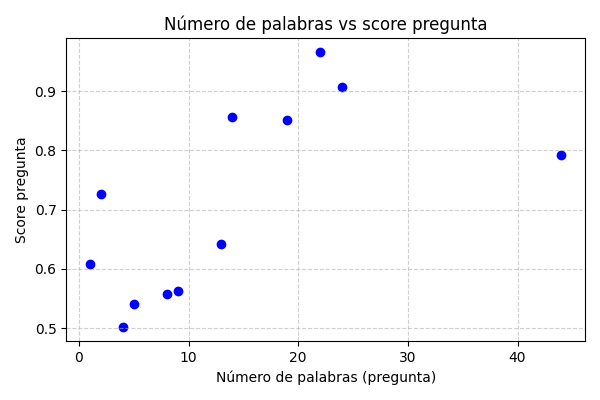
\includegraphics[width=0.7\textwidth]{../graficos/scatter_pregunta.png}
\caption{Dispersión entre número de palabras y score para preguntas}
\end{figure}

\begin{figure}[H]
\centering
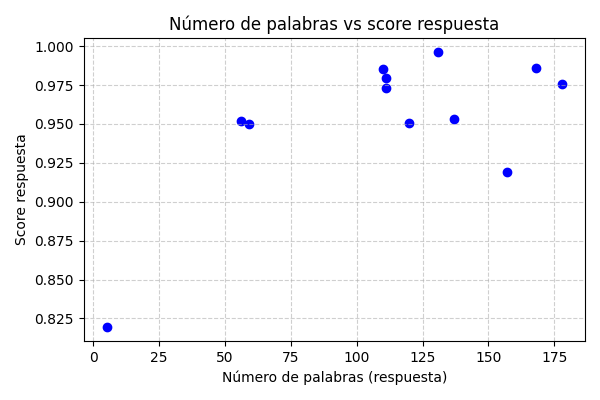
\includegraphics[width=0.7\textwidth]{../graficos/scatter_respuesta.png}
\caption{Dispersión entre número de palabras y score para respuestas}
\end{figure}

\end{document}
